\documentclass{article}
\usepackage{amsmath}
\usepackage{graphicx}
\usepackage{geometry}
\geometry{a4paper, portrait, margin=1in}
\setlength\parindent{0pt}
\begin{document}

\begin{Large}
    \textbf{Project Plan} \\
\end{Large}

\begin{large}
    \texttt{\today} $\vert$ \textit{Our tasks, milestones and Gantt Chart} \\
\end{large}

\pagenumbering{gobble}


\textsf{\textbf{Y4:}} \text{Adam, Alejandro, Ammar, Brendan, Dakshit, Joshua, Marek}\\
\textsf{\textbf{Tutor:}} \text{Dr Mustafa}


\vspace{1em}
\hrule
\vspace{1.5em}

\textbf{MVP Features}

\begin{enumerate}
    \item Occupancy information and heatmap (GET request)
    \item Report crowd level (POST request)
    \item Integrate user reports (Algorithm and PUT request)
    \item Calendar and study time feature (GET request)
    \item Save user study time blocks (PUT requset)
\end{enumerate}

\textbf{Secondary Features}

\begin{enumerate}
    \setcounter{enumi}{5}
    \item Location suggestion
    \item Find a study buddy pairing (Algorithm)
    \item .ics calendar upload feature (PUT request)
    \item Study buddy DM chat feature
\end{enumerate}

\textbf{Extra Features}
\begin{enumerate}
    \setcounter{enumi}{9}
    \item Location services (foreground)
\end{enumerate}

\textbf{Ambitious Features}
\begin{enumerate}
    \setcounter{enumi}{10}
    \item Native mobile apps for background location services
\end{enumerate}

\textbf{Gantt Chart}

    \begin{center}
        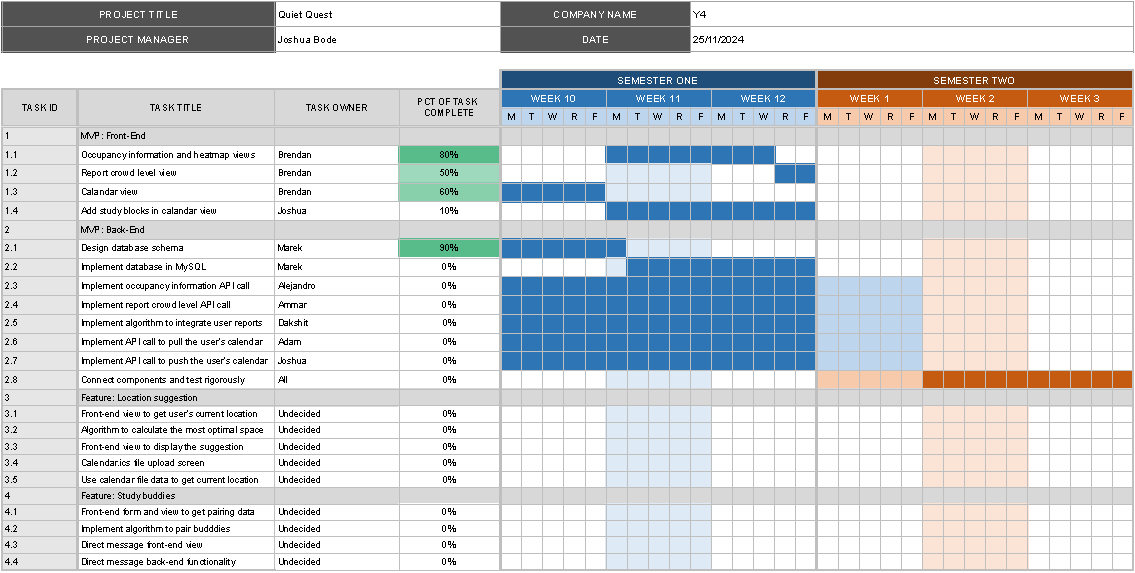
\includegraphics[height=120px, page=1]{mini-gantt-crop.pdf} \\
        \includegraphics[height=150px, page=2]{mini-gantt-crop.pdf}
    \end{center}



\end{document}